\documentclass[12pt]{article}
\usepackage{color}
\usepackage{graphicx}
\usepackage{booktabs}
\usepackage{amsmath}
\usepackage[utf8]{inputenc}
%\usepackage[german]{babel}
\usepackage{multirow}
%\usepackage{siunitx}
\usepackage{pbox}
%\usepackage{tabularx}
\usepackage{multirow}
\usepackage{float}
\usepackage{amssymb,amsmath}
\makeatletter
\def\maketag@@@#1{\hbox{\m@th\normalfont\normalsize#1}}
\makeatother
\setlength{\parindent}{0pt}

%\addtolength{\textwidth}{1in}
%\addtolength{\textheight}{1in}
%\addtolength{\evensidemargin}{0.5in}
%\addtolength{\oddsidemargin}{-0.5in}
%\addtolength{\topmargin}{-0.6in}
%\addtolength{\bottommargin}{0.4in}


\usepackage[top = 2.50cm, bottom = 2.50cm, left = 2.75cm, right = 2.50cm]{geometry}

\renewcommand{\floatpagefraction}{1.0}


\begin{document}
\title{PHY118/119 \\ {\bf Übungsstunde 1, Kinematik}}
\author{Assistent: Simon Flury \\E-mail: simon.flury@uzh.ch\\\\ }
\maketitle

\section{Wichtig!!!}
Dieses Dokument ist kein offizielles Dokument, es ist weder von Prof.Kilminster noch vom Hauptassistenten abgesegnet, somit kann sich nicht darauf bezogen werden und es wird auch keine Haftung für Fehler übernommen. Es dient einzig und allein als Lernunterstützung von mir an euch und bezieht sich ausschliesslich auf meine Übungsstunde.
\section{Beschreibung und theoretischer Hintergrund}
In  den ersten beiden Serien geht es um kinematische Probleme. Die Kinematik ist ein Teil der Physik, welcher sich mit der Bewegung von Objekten und somit der Beschreibung ihrer Trajektorien befasst.\\
\\ Nach den üblichen Konventionen wird der Ort mit S bzw. x, die Geschwindigkeit mit v und die Beschleunigung mit a bezeichnet. Diese grössen sind abhängig von der Zeit, dementsprechenden sind es Funktionen welche von t abhängen $x(t), v(t), a(t)$.Ort,Geschweindigkeit und Beschleunigung stehen in direktem Zusammenhang und lassen sich, durch differenzieren oder integrieren nach der Zeit, direkt ineinander überführen

\begin{equation}
\begin{split}
\dfrac{d}{dt} x(t) + x_0 = v(t) \rightarrow x(t) + x_0 = \int v(t) dt \\
\dfrac{d}{dt} v(t)+v_0 = a(t) \rightarrow v(t)+v_0 = \int a(t) dt
\end{split}
\end{equation}
wobei die Grössen $x_0$ (Startpunkt) und $v_0$ (Anfangsgeschwindigkeit) Konstanten sind, welche durch die Anfangsbedingungen (eure Aufgabenstellung) gegeben werden. Durch diesen Zusammenhang lassen sich die folgenden Formeln herleiten:
\begin{equation}
\begin{split}
S = x(t) = x_0 + vt+\dfrac{at^2}{2} \\
v = v_0 + at \\
v^2-v_0^2 = 2aS \\
\bar{v} = \dfrac{\Delta x}{\Delta t} = \dfrac{x_2-x_1}{t_2-t_1} \\
\bar{a} = \dfrac{\Delta v}{\Delta t} = \dfrac{v_2-v_1}{t_2-t_1}
\end{split}
\end{equation}
Mit $\bar{v}, \bar{a}$ wird die Durchschnittsgeschwindigkeit und Durchschnittsbeschleunigung bezeichnet. Anders als zuvor ergeben sich diese nicht durch Differentation, sprich aus der Steigung der Tangenten, sonders aus der Steigung der Sekanten.
Aus diesen einfachen Formeln ergeben sich für die folgenden Spezialfälle diese Zusammenhänge:\\
\\ Freier Fall:
\begin{equation}
\begin{split}
h = \dfrac{gt^2}{2} \\
v = \sqrt{2hg}
\end{split}
\end{equation}
In diesem Fall wirkt nur die Gravitation also wird das Objekt mit $g = 9.81 m/s^2$ nach unten beschleunigt. Nun stellt sich natürlich die Frage nach dem Vorzeichen von $g$. Dies hängt ganz davon ab wie ihr euer Koordinatensystem definiert  (wir wählen unser System immer so dass $g$ negativ ist). Betrachtet dazu die Aufgabe 2 in der Serie 2. Es gibt nun zwei Möglichkeiten euren Nullpunkt zu definiere: Wählt ihr den Balkon als Nullpunkt, dann ist $g$ negativ sowie $h$ auch, denn der Boden liegt nun in eurem koordinatensystem bei $y=-h$. Wählt ihr den Boden als Nullpunkt ist $g$ ebenfalls negativ der Balkon auf Höhe $h$, die Gleichung für $y$ sieht nun jedoch ein wenig anders aus, da ihr ja das Objekt von der Höhe $h$ fallen lässt, somit habt ihr eine Starthöhe, damit gilt $y(t) = 0 = h_0+\dfrac{(-g)t^2}{2}$.\\
\\ Senkrechter Wurf nach oben:
\begin{equation}
\begin{split}
h = h_0 + v_0t-\dfrac{gt^2}{2} \\
v = v_0 - gt
\end{split}
\end{equation}
Wie schon zu Beginn erklärt sind die mit dem Index 0 bezeichneten Grössen Konstanten, wie Anfangsgeschwindigkeit oder Starthöhe. In diesem Fall wirkt die Gravitationsbeschleunigung der Startgescwindigkeit entgegen, bis diese sich gegenseitig aufheben. Dies ist der Fall bei der maximalen Steighöhe, dort gilt $v=0$ bzw.$ v_0t + (-g)t = 0$ was gleichbedeutend ist mit $\dfrac{d}{dt} x(t) = 0$ was eine Extremalstelle definiert. Nach erreichen dieses Punktes geht es über in einen ganz normalen freien Fall.\\
\\
Waagrechter Wurf:

\begin{equation}
\begin{split}
h = \dfrac{gt^2}{2} \\
s = vt
\end{split}
\end{equation}
Augfrund der Gravitation wird das Objekt nach unten (-y Richtung) beschleunigt und erhält somit eine nicht konstante Geschwindigkeitskomponente $v_y = gt$. Die vertikale Distanz ($\Delta y)$ wird mit der Höhe assoziert. Die Distanz in x-Richtung (s) ist gegeben durch die Anfangsgeschwindigkeit mal die Zeit und somit von der Gravitationsbeschleunigung unbeeinflusst.\\
\\
Schiefer Wurf:
\begin{equation}
\begin{split}
x_w = \dfrac{v_0^2 \cdot sin(2\alpha)}{g} \\
v_y = v \cdot sin(\alpha)-gt \\
v_x = v \cdot cos(\alpha) \\
v = \sqrt{v_x^2 + v_y^2} \\
y = x \cdot tan(\alpha)-\dfrac{gx^2}{2v_0^2cos(\alpha)^2}
\end{split}
\end{equation}
dabei bezeichnet $x_w$ die Wurfweite spricht die Distanz in x-Richtung $\Delta x$ und $y$ die Wurfhöhe an der Stelle $x$.
Der schiefe Wurf ist eine Kombination der vorherigen Fälle. Auch er enthält eine maximale Steighöhe in der jedoch nicht $v = 0$ sonder $v_y = 0$ gilt, da wiederum die Gravitationsbeschleunigung nur die y-Komponente beeinflusst. Dies bedeutet, die Extremalstelle zeichnet sich durch $\dfrac{d}{dt} v_y = 0$ aus. Durch die trigonometrischen Funktionen ergeben sich jeweils mehrere Lösungen, aufgrund der Periodizität der Funktionen.

\section{Messungen und Messfehler}
Jede Messung ist Fehlerbehaftet, dass bedeutet das mit jeder Messgrösse eine bestimmte Unsicherheit einhergeht. Ein Messergebnis ohne Angabe der Messunsicherheit ist somit wertlos!\\
Schreibweise: (Messergebnis +/- Messunsicherheit) Einheit \\
Ergebnis und Unsicherheit müssen die gleiche Anzahl Stellen haben z.B. $v = (1.08 \pm 0.10) \dfrac{m}{s}$ und nicht $v=(1.08 \pm 0.1) \dfrac{m}{s}$.\\
\\Es gibt zwei Arten von Messunsicherheiten, systematische und statistische. Systematische Fehler kommen zum Beispiel durch eine falsche Eichung der Messgeräte zustande. Sie zeichen sich dadurch aus, dass die Abweichungen bei Wiederholung der Messung unter gleichen Bedingungen immer gleich sind. Statistische Fehler sind zufällige Fehler und zeichnen sich dadurch aus, dass bei Wiederholung der Messung die Abweichungen immer anders sind. Nur diesen Fehler können wir mit statistischen Methoden Rechnung tragen.\\
\\In der Aufgabe 5 vom Blatt 1 wurde euch eine Unsicherheit auf eine Messgrössen gegeben $\Delta x = 1cm$. Hierbei handelt es sich um einen statistischen Messfehler. Ihr wisst nun dass ihr mit der Formel $\dfrac{\Delta v}{v} = \dfrac{\Delta x}{x}$ den Fehler auf die Geschwindigkeit berechnen könnt. Hättet ihr zudem noch einen Fehler auf die Zeit, könntet ihr diesen Fall analog zum ersten berechnen, mit zusätzlichem Zeitterm $\dfrac{\Delta v}{v} = \dfrac{\Delta x}{x} + \dfrac{\Delta t}{t}$\\
\\ Ich möchte an dieser Stelle nicht weiter auf die Berechnung von Fehlern eingehen, da dies uns sofort auf die Gauss'sche Fehlerfortpflanzung führen würde, wofür wir aber erst partielle Ableitungen einführen müssten. Dies möchte ich jedoch erst machen, wenn Prof.Kilminster in der Vorlesung dieses Konzept einführt.


\section{Differentialrechnung}
Hier möchte ich nochmals eine kleine Zusammenfassung geben, welche für diese Vorlesung sicher ausreichen sollte.\\
\\
Eine Funktion heisst differenzierbar an der Stelle $x_0$, wenn gilt:

\begin{equation}
\lim_{x \to \ x_0} \dfrac{f(x)-f(x_0)}{x-x_0} = \lim_{h \to \ 0} \dfrac{f(x_0+h)-f(x_0)}{h}
\end{equation}

wobei $h = x-x_0$\\
\\ Die geometrische bedeutung der Ableitung ist die Steigung der Tangente am Punkt $x_0$.
\subsection{Regeln}
Konstante Funktion:
\begin{equation}
(a)' = 0
\end{equation}
Faktorregel:
\begin{equation}
(a \cdot f)' = a \cdot f'
\end{equation}
Summenregel:
\begin{equation}
(g \pm h)' = g' \pm h'
\end{equation}
Produktregel:
\begin{equation}
(g\cdot h)' = g' \cdot h + g \cdot h'
\end{equation}
Quotientenregel:
\begin{equation}
\left(\dfrac{g}{h}\right)' = \dfrac{g' \cdot h-g \cdot h'}{h^2}
\end{equation}
Potenzregel:
\begin{equation}
(x^n)' = nx^{n-1}
\end{equation}
Kettenregel:
\begin{equation}
(g \circ h)'(x) = (g(h(x)))' = g'(h(x)) \cdot h'(x)
\end{equation}
\begin{figure}[H]
  \centering{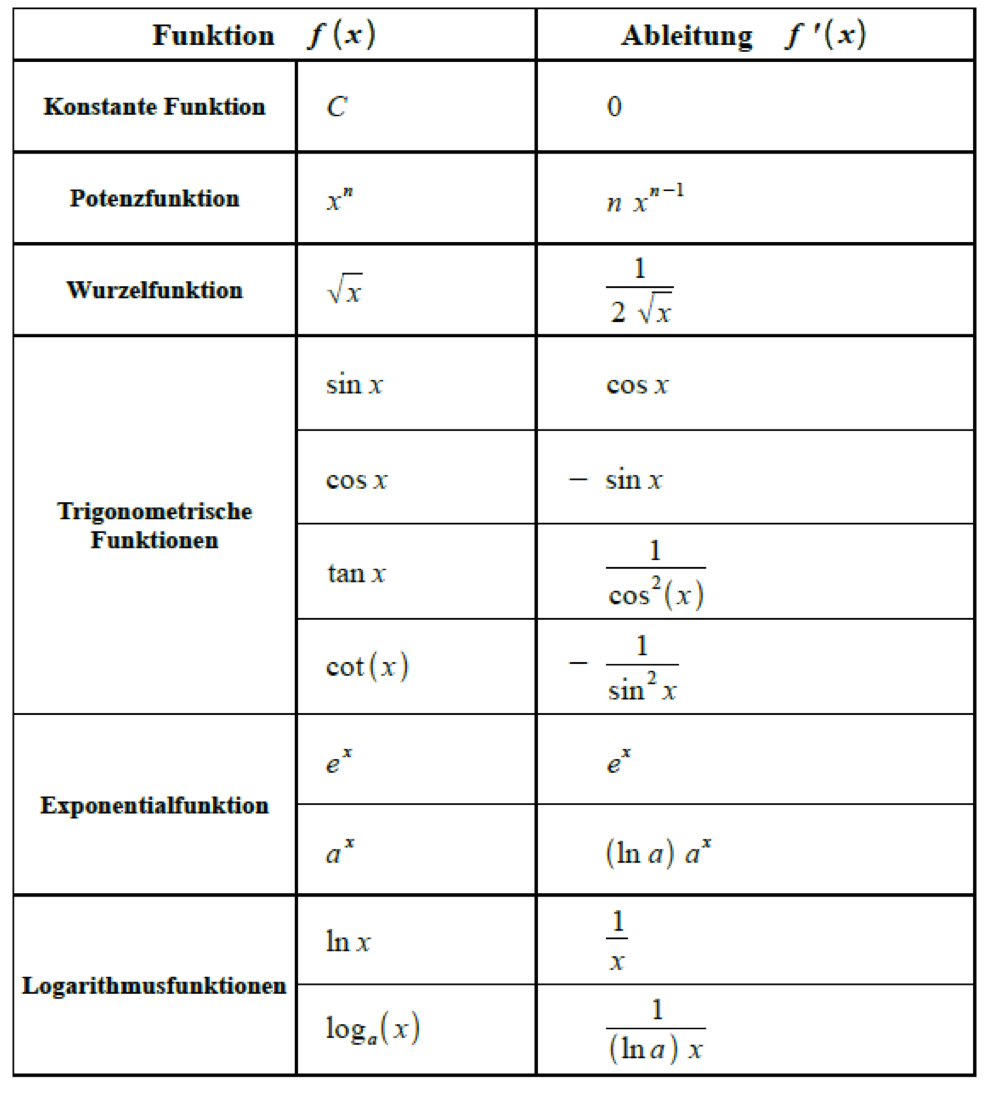
\includegraphics[width=0.95\textwidth]{Ableitungen.png}}
  \caption{Wichtige Ableitungen, welche ihr auswendig kennen solltet.}
  \label{fig:1teil}
\end{figure} 

Beispiele:
\begin{equation}
y = arctan(x) \cdot ln(x)
\end{equation}
\begin{equation}
y' = arctan'(x) \cdot ln(x) + arctan(x) \cdot ln'(x) = \dfrac{1}{1+x^2} \cdot ln(x) + arctan(x) \cdot \dfrac{1}{x}
\end{equation}
\begin{equation}
y = \dfrac{2x^2 + 3}{8x + 1} 
\end{equation}
\begin{equation}
y' = \dfrac{(2x^2+3)' \cdot (8x+1)-(2x^2 + 3) \cdot (8x+1)'}{(8x+1)^2}
\end{equation}
\begin{equation}
y = (1+cos(2x))^2
\end{equation}
\begin{equation}
y' = 2(1+cos(2x)) \cdot (1+cos'(2x)) \cdot (2x)' = 2(1+cos(2x)) \cdot (-sin(2x)) \cdot 2 = -4(1+cos(2x)) \cdot sin(2x)
\end{equation}

\section{Integralrechnung}
Wir verwenden hier das sogennate Riemann-Integral. Dieses ist definiert als Riemann-Summe:
\begin{equation}
\int_{a}^b f(x)\, \mathrm{dx} = \lim_{n \to \ \infty } \sum\nolimits_{i=1}^n f(x_i) \Delta x
\end{equation}
was geometrisch gesehen einfach die Fläche unter der Kurve, approximiert als Summe von Rechtecken mit der Höhe $f(x_i)$ und der Breite $\Delta x$, darstellt.
\subsection{Sätze und Definitionen}
\begin{equation}
\int_{b}^b f(x)\, \mathrm{dx} = 0 \ \ \mathrm{and} \int_{b}^c f(x)\, \mathrm{dx} = -\int_{c}^b f(x)\, \mathrm{dx}
\end{equation}
Intervalladditivität:
\begin{equation}
\int_{a}^b f(x)\, \mathrm{dx} = \int_{a}^c f(x)\, \mathrm{dx} + \int_{c}^b f(x)\, \mathrm{dx}
\end{equation}
Hauptsatz der Differential- und Integralrechnung:\\
\\ Seien $f\colon I \to R$ stetig und $a \in I$. Dann ist die Integralfunktion zu $a$ 
$F_a\colon I \to R, \ \ x \mapsto \int_{a}^x f(x)\, \mathrm{dx}$
differenzierbar und es gilt $F_a'(x) = f(x) \ \ \forall x \in I$\\
\\ Stammfunktion: Eine Funktion $F$ heisst Stammfunktion der Funktion $f$, wenn $F' = f$ gilt.\\
\\ Ist $F$ eine Stammfunktion von $f$, dann gilt: $G$ ist Stammfunktion von $f \Leftrightarrow  \exists c \in R : G(x) = F(x) +c$\\
(dies bedeutet einfach, dass eure Stammfunktion nur bis auf eine Konstante bestimmt ist).\\
\\ Das Integral $\int f(x) dx := G(x)$ ist das unbestimmte Integral von $f$\\
\\Nach dem Hauptsatz gilt: Ist $F$ eine Stammfunktion von $f$, so gilt
\begin{equation}
\int_{a}^b f(x)\, \mathrm{dx} = F(b)-F(a)
\end{equation}
Summen und Faktoregel:
\begin{equation}
\int_{a}^b f(x) + g(x)\, \mathrm{dx} = \int_{a}^b f(x)\, \mathrm{dx} + \int_{a}^b g(x)\, \mathrm{dx}
\end{equation}
\begin{equation}
\int_{a}^b cf(x)\, \mathrm{dx} = c \int_{a}^b f(x)\, \mathrm{dx}
\end{equation}
Substitutionsregel:
\begin{equation}
\int_{a}^b f( \varphi (x)) \cdot \varphi'(x) \, \mathrm{dx} = \int_{\varphi(a)}^{\varphi(b)} f(x)\, \mathrm{dx}
\end{equation}
Beispiel:\\
$\int_{3}^5 \dfrac{2x}{(1+x^2)^2}\, \mathrm{dx}$\\
Vorgehen: 1. Im Integranden einen Term $\varphi(x)$ suchen, dessen Ableitung $\varphi(x)'$ ebenfalls im Integranden enthalten ist. In diesem Beispiel ist es der Term $\varphi(x) = 1+x^2$ und $\varphi'(x) = 2x$.\\
2. erkenne die Funktion $f$ im Integranden, so dass $f(\varphi(x)) \cdot \varphi(x)'$ der Integrand ist. In unserem Beispiel also $f(x) = \dfrac{1}{x^2} \rightarrow f(\varphi(x)) \cdot \varphi(x)' = \dfrac{1}{(1+x^2)^2} \cdot 2x = \dfrac{2x}{(1+x^2)^2}$ damit wird unser Integral zu $\int_{10}^{26} \dfrac{1}{x^2}\, \mathrm{dx} = -\dfrac{1}{x} \mid_{10}^{26} = \dfrac{4}{65}$\\
\\
Partielle Integration:
\begin{equation}
\int_{a}^b f(x) \cdot g(x)\, \mathrm{dx} = f(x)G(x) \mid_a^b - \int_{a}^b f'(x)G(x)\, \mathrm{dx}
\end{equation}
dabei ist $G(x)$ die Stammfunktion von $g(x)$\\
\\ Beispiel\\
$\int_{0}^{\pi} x \cdot sin(x)\, \mathrm{dx} = x \cdot (-cos(x)) \mid_0^{\pi} - \int_{0}^{\pi} 1 \cdot (-cos(x))\, \mathrm{dx} = x \cdot (-cos(x)) \mid_0^{\pi} - (-sin(x)) \mid_0^{\pi} = \pi$\\
\\
\begin{figure}[H]
  \centering{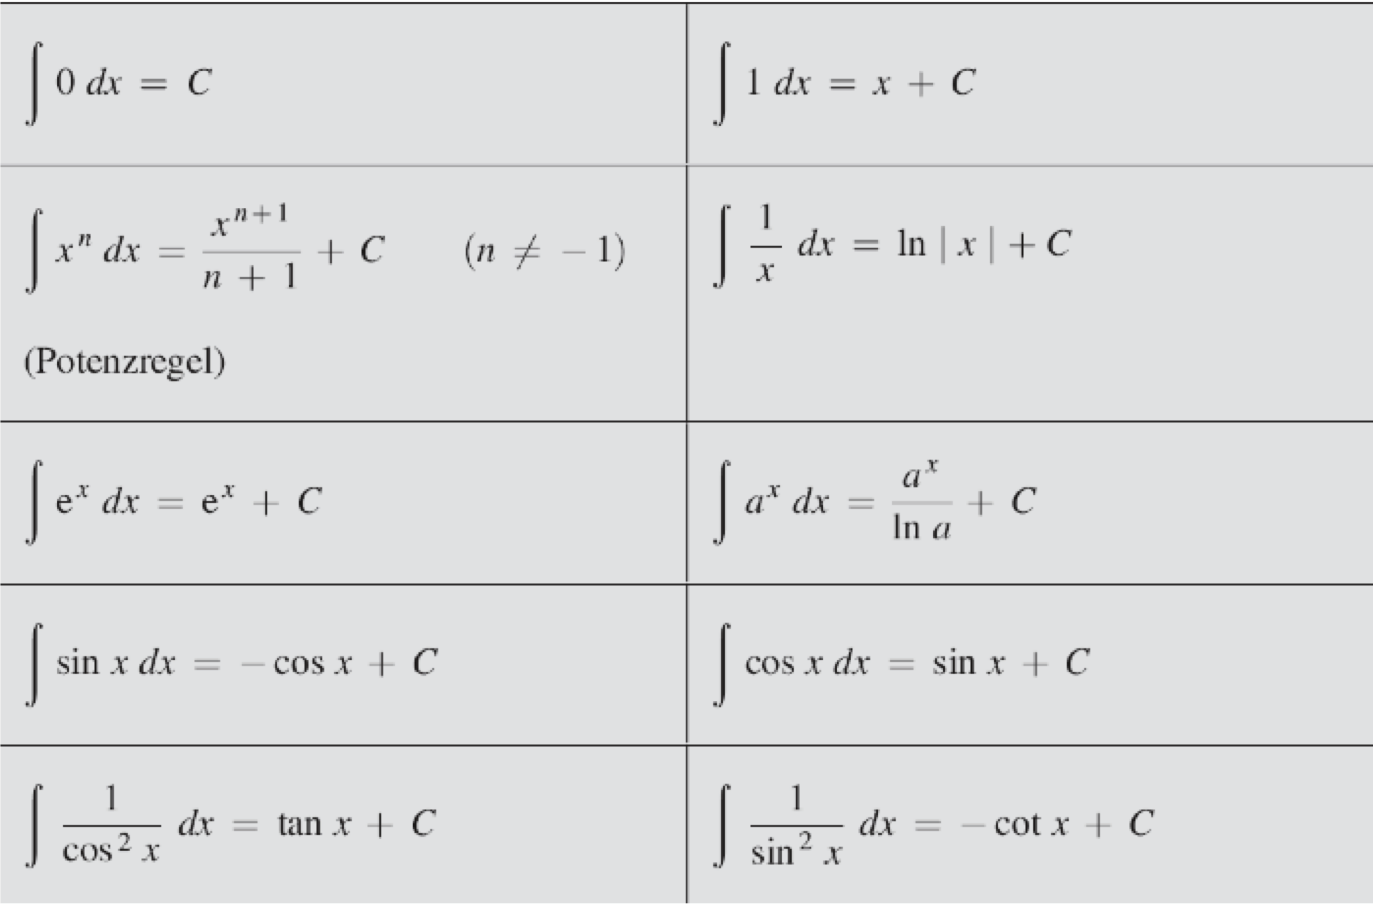
\includegraphics[width=0.8\textwidth]{Integral.png}}
  \caption{Wichtige Integrale bzw. ihre Stammfunktionen..}
  \label{fig:1teil}
\end{figure} 

\section{Lösung der Piratenschiff-Aufgabe}
\begin{figure}[H]
  \centering{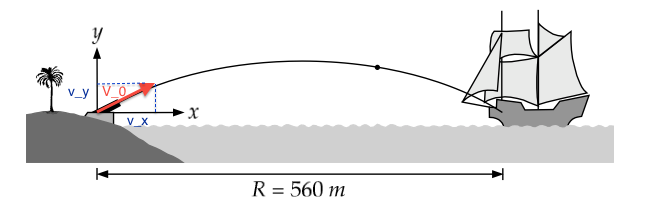
\includegraphics[width=0.8\textwidth]{Piratenaufgabe.png}}
  \caption{Situation.}
  \label{fig:1teil}
\end{figure}
Auf welchen Winkel muss die Kanone eingestellt werden, damit das Schiff getroffen wird?\\
Lösung:\\
Wir haben die Startgeschwindigkeit $v_0$ der Kugel gegeben sowie die Distanz in x-Richtung, $R = 560m$. Für die Geschwindigkeitskomponenten in x- und y-Richtung gelten folgende Relationen:
\begin{equation}
\begin{split}
v_x = v_0 \cdot cos(\alpha) \\
v_y = v_0 \cdot sin(\alpha)
\end{split}
\end{equation}
Diese Situation beschreibt genau einen schiefen Wurf, dabei gilt wie schon erklärt die Geschwindigkeit in x-Richtung ist konstant, da nur die Komponente in y-Richtung eine Änderung durch die Erdbeschleunigung $g$ erfährt. Dies bedeutet, dass folgendes für x,y Koordinaten gilt (x beschreibt horizontale Distanz, y vertikale sprich die Höhe):
\begin{equation}
\begin{split}
x = v_xt \\
y = \dfrac{(-g)t^2}{2} + v_yt
\end{split}
\end{equation}
auch hier haben wir wieder $g$ negativ gewählt da die Gravitation die Kugel nach unten beschleunigt. Was wir nun haben ist ein sogenanntes Gleichungssystem bestehend aus zwei Gleichungen. Setzen wir unsere Bedingungen ein, also schreiben für $t=t'$ die Zeit nach der das Schiff getroffen wird, setzen $x=R$ da dies die horizontale Entfernung des Schiffes ist und $y=0$ da die Kugel das Schiff auf Höhe der Kanone trifft (vereinfachte Annahme) also dort wo wir (praktischerweise) unseren Koordinatenursprung (Nullpunkt) festgelegt haben. Dies ins Gleichungssystem eingesetzt führt aus das neue Gleichungssystem:
\begin{equation}
\begin{split}
R = v_0 \cdot cos(\alpha)t' \\
0 = \dfrac{(-g)t'^2}{2} + v_0 \cdot sin(\alpha)t'
\end{split}
\end{equation}
Nun Lösen wir die erste Gleichung nach $t'$ auf:
\begin{equation}
t' = \dfrac{R}{v_0cos(\alpha)}
\end{equation}
Jetzt können wir $t'$ in die zweite Gleichung einsetzen:
\begin{equation}
\dfrac{gR}{2v_0cos(\alpha)} = v_0sin(\alpha) \rightarrow \dfrac{gR}{2} = v_0^2sin(\alpha)cos(\alpha)
\end{equation}
Unter verwendung der trigonometrischen Identität $2cos(\alpha)sin(\alpha) = sin(2\alpha)$ bekommt ihr
\begin{equation}
\dfrac{gR}{2} = v_0^2sin(\alpha)cos(\alpha) = \dfrac{1}{2} \cdot v_0^2sin(2\alpha) \rightarrow 2\alpha = arcsin \left(\dfrac{gR}{v_0^2} \right)
\end{equation}
Wie schon zu Beginn erläutert erhält man zwei Lösungen für $\alpha$ aufgrund der Periodizität der trigonometrischen Funktionen.
\end{document}

